\documentclass[a4paper,french,bookmarks]{article}

\usepackage{./Structure/4PE18TEXTB}

\newboxans
\usepackage{booktabs}

\begin{document}

    \renewcommand{\thesection}{\Roman{section}} 
    \renewcommand{\thesubsection}{\thesection.\Alph{subsection}}
    \setlist[enumerate]{font=\color{white5!60!black}\bfseries\sffamily}
    \renewcommand{\labelenumi}{\thesection.\arabic{enumi}.}
    \renewcommand*{\labelenumii}{\alph{enumii}.}
    \renewcommand*{\labelenumiii}{\alph{enumiii}.}
    
    \stylizeDocSpe{Physique}{Devoir maison n° 8}{}{Pour le mercredi 5 décembre 2022}
    
    \section{Premier problème}
    
    \subsection{Impédance d'une corde}
    
    On considère une corde sans raideur (n'opposant aucune résistance à la déformation), de masse linéique $\mu$ et tendue à la tension $T_0$ lorsqu'elle est au repos. On néglige le poids de la corde par rapport à la tension du fil et on s'intéresse aux petits mouvements verticaux de la corde.
    
    \begin{enumerate}
        \itt Les calculs seront tous fait de manière approchée, au premier ordre en $\dfrac{\partial y}{\partial x}$.
        
        \itt Un point $M$, situé à l'abscisse $x$ lorsque la corde est au repos, s'est déplacé de $y\p{x, t}$ selon $\p{O, \vec{u_y}}$ :
    \end{enumerate}
    %
    \begin{center}
        \begin{tikzpicture}
            \begin{axis}[
                clip                =   true,
                axis lines          =   middle,
                    %minor tick num      =   4,
                    domain              =   0:53,
                    %xtick distance      =   1,
                    %ytick distance      =   1,
                    trig format plots   =   rad,
                    trig format         =   rad,
                    xlabel              =   {$\vec{u_x}$},
                    ylabel              =   {$\vec{u_y}$},
                    xmin                =   0,
                    xmax                =   10,
                    ymin                =   -1.8,
                    ymax                =   1.8,
                    width               =   15cm,
                    height              =   6cm,
                    grid                =   none,
                    xtick               =   {0, 2},
                    ytick               =   {-sin(4)},
                    xticklabels         =   {$O$, $x$},
                    yticklabels         =   {$y\p{t, x}$}
                ]
                    \addplot[color=main3,very thick,samples=500,smooth,domain=0:10] {-sin(\x+2)};
                    \addplot[color=main3,opacity=0.5,thick, densely dotted,samples=500,smooth,domain=0:10] {-sin(\x+1.85)};
                    \addplot[color=main3,opacity=0.3,thick, densely dotted,samples=500,smooth,domain=0:10] {-sin(\x+1.7)};
                    \addplot[color=main3,opacity=0.1,thick, densely dotted,samples=500,smooth,domain=0:10] {-sin(\x+1.55)};
                    
                    \draw [main1, dashed] (2, 0.76) -- (2, 0);
                    
                    \draw [main1, dashed] (0, 0.76) -- (3, 0.76);
                    \addplot[color=main1,thick,samples=500,smooth,domain=1:3] {-cos(4)*(\x - 2) - sin(4)};
                    
                    
                    \coordinate (m) at (2, 0.76);
                    \coordinate (a) at (3, 0.76);
                    \node[label={[font=\footnotesize,main1,fill=white,fill opacity=0.7,text opacity=1]right:$\alpha\p{x, t}$}] at (2.6, 0.95) {};
                    \coordinate (b) at (3, 1.41);
                \end{axis}
                
                \pic [draw=main1, thick, ->, angle eccentricity=-1.5,angle radius=1cm] {angle = a--m--b};
        \end{tikzpicture}
    \end{center}
    
    Chaque élément de la corde est soumis à des forces de tension tangentes en tout point à la corde. On note $\vec{T}\p{x, t}$ la tension qu'exerce à un instant $t$ la partie de la corde d'abscisse supérieure à $x$ sur la partie de la corde d'abscisse inférieure à $x$. On note $\alpha\p{x, t}$ l'angle que fait la tangente à la corde au point $x$ à l'instant $t$ avec l'horizontale.\medskip
    
    Avec les hypothèses de travail, on a dans la base $\p{O, \vec{u_x}, \vec{u_y}}$ :
    %
    \[ \vec{T}\p{x, t} = \p{\begin{array}{c}
        T_x\p{x, t} \\
        T_y\p{x, t}
    \end{array}} \approx \p{\begin{array}{c}
        T_0 \\
        T_0\alpha\p{x, t}
    \end{array}}\]
    %
    La progression d'une onde sur cette corde s'accompagne d'un couplage entre $T_y\p{x, t}$, \guill{cause} du mouvement de la corde et $v\p{x, t}$, \guill{conséquence} :
    %
    \[ \left\lbrace\begin{array}{rl}
        v\p{x, t} &= \dfrac{\partial y\p{x, t}}{\partial t} \\[4pt]
        T_y\p{x, t} = T_0\alpha\p{x, t} &= T_0\dfrac{\partial y\p{x, t}}{\partial x} 
    \end{array}\right.\]
    %
    On considère une onde plane progressive telle que $y_+\p{x, t} = f\p{t - \dfrac{x}{c}}$ avec $c = \sqrt{\dfrac{\tau_0}{\mu}}$.
    
    \begin{enumerate}
        \item Donner la définition d'une onde progressive. Que signifie la grandeur $c$ ?
        
        \boxansconc{
            On appelle \emph{onde progressive} une grandeur physique intensive variant \emph{spatiellement} et \emph{temporellement} de \emph{proche en proche}. La grandeur $c$ (célérité) représente la vitesse de propagation (spatiale) de l'onde.
        }
        
        \item Exprimer le champ des vitesses verticales $v_+\p{x, t}$ associé à $y_+\p{x, t}$, en fonction de $f'\p{u}$ où
        %
        \[ f' = \dfrac{\dif f}{\dif u} \qquad\et\qquad u = \p{t - \dfrac{x}{c}} \]
        
        \boxansconc{
            \[ v_+\p{x, t} = \dfrac{\partial y_+\p{x, t}}{\partial t} = \dfrac{\partial y_+\p{x, t}}{\partial u}\dfrac{\partial u}{\partial t} = \dfrac{\partial f\p{t - \dfrac{x}{c}}}{\partial u}\dfrac{\partial u}{\partial t} = \dfrac{\partial f\p{u}}{\partial u}\dfrac{\partial \p{t - \dfrac{x}{c}}}{\partial t} = f'\p{u}\times 1\]
            %
            Donc $v_+\p{x, t} = f'\p{t - \dfrac{x}{c}}$.
        }
        
        \newpage
        
        \item Établir l'expression de la composante transversale $T_{y+}\p{x, t}$ associée à $y_+\p{x, t}$ en fonction de $c$, $T_0$ et $f'$.
        
        \boxansconc{
            Similairement à la question précédente :
            %
            \[ T_{y+}\p{x, t} = T_0\dfrac{\partial y_+\p{x, t}}{\partial x} = T_0\dfrac{\partial f\p{u}}{\partial u}\dfrac{\partial u}{\partial x} = T_0f'\p{u}\times \p{-\dfrac{1}{c}} = -\dfrac{T_0}{c}f'\p{t - \dfrac{x}{c}}\]
        }
    \end{enumerate}
    
    On définit l'impédance $Z$ de la corde par la relation $T_{y+}\p{x, t} = -Zv_+\p{y, t}$ avec $Z \in \bdRp$ une constante réelle ne dépendant que de $T_0$ et de $\mu$.
    
    \begin{enumerate}[resume]
        \item Obtenir l'expression de $Z$ en fonction de $T_0$ et de $\mu$.
        
        \boxansconc{
            On a $Z = -\dfrac{T_{y+}\p{x, y}}{v_+\p{x, y}} = -\dfrac{-\dfrac{T_0}{c}f'\p{u}}{f'\p{u}} = \dfrac{T_0}{c}$. On a bien $Z = \dfrac{T_0}{c} > 0$.
        }
        
        \item Montrer que si l'on considère une onde progressive $y_-\p{x, t} = g\p{t + \dfrac{x}{c}}$, on a alors $T_{y-}\p{x, t} = Z{v_-}\p{x, t}$.
        
        \noafter
        %
        \boxans{
            Posons $v = t + \dfrac{x}{c}$ et $g' = \dfrac{\dif g}{\dif v}$. On a 
            %
            \[ v_-\p{x, t} = \dfrac{\partial y_-\p{x, t}}{\partial t} = \dfrac{\partial y_-\p{x, t}}{\partial v}\dfrac{\partial v}{\partial t} = \dfrac{\partial g\p{t - \dfrac{x}{c}}}{\partial v}\dfrac{\partial v}{\partial t} = \dfrac{\partial g\p{v}}{\partial v}\dfrac{\partial \p{t + \dfrac{x}{c}}}{\partial t} = g'\p{u}\times 1\]
            %
            D'où $v_-\p{x, t} = g'\p{v}$. De même :
            %
            \[ T_{y-}\p{x, t} = T_0\dfrac{\partial y_-\p{x, t}}{\partial x} = T_0\dfrac{\partial g\p{v}}{\partial v}\dfrac{\partial v}{\partial x} = T_0g'\p{u}\times \p{\dfrac{1}{c}} = \dfrac{T_0}{c}f'\p{u}\]
            %
        }
        %
        \nobefore\yesafter
        %
        \boxansconc{
            On a bien $T_{y-}\p{x, t} = \dfrac{T_0}{c}{v_-}\p{x, t}$, c'est-à-dire $T_{y-}\p{x, t} = Z{v_-}\p{x, t}$.
        }
        %
        \yesbefore
    \end{enumerate}
    
    \subsection{Réflexion entre deux cordes}
    
    On considère deux cordes semi-infinies :
    %
    \begin{enumerate}
        \itt la première, d'impédance $Z_1$, s'étend de $x = -\infty$ à $x = 0$ ;
        
        \itt la seconde, d'impédance $Z_2$, s'étend de $x = 0$ à $x = +\infty$.
    \end{enumerate}
    
    \begin{center}
        \begin{tikzpicture}
            \begin{axis}[
                clip                =   true,
                axis lines          =   middle,
                    %minor tick num      =   4,
                    domain              =   0:53,
                    %xtick distance      =   1,
                    %ytick distance      =   1,
                    trig format plots   =   rad,
                    trig format         =   rad,
                    xlabel              =   {$\vec{u_x}$},
                    ylabel              =   {$\vec{u_y}$},
                    xmin                =   0,
                    xmax                =   10,
                    ymin                =   -1.5,
                    ymax                =   1.8,
                    width               =   15cm,
                    height              =   4.5cm,
                    grid                =   none,
                    xtick               =   {5},
                    ytick               =   {0},
                    xticklabels         =   {$O$},
                    yticklabels         =   {$\text{}$}
                ]
                    \addplot[color=main3,very thick,samples=500,smooth,domain=0:5] {sin(\x+2) + 0.3*sin(3*\x - 2)};
                    
                    \node[main3] at (2.45, -0.8) {$Z_1$};
                    
                    \addplot[color=main5,very thick,samples=500,smooth,domain=5:10] {0.3*sin(\x+2.4) + 0.5*sin(3*\x - 2.4)+0.5};
                    
                    \node[main5] at (7.5, 1.1) {$Z_2$};
                    
                    \draw [main1, dashed] (5, 0) -- (5, 0.76);
                \end{axis}
        \end{tikzpicture}
    \end{center}
    
    Une onde incidente est envoyée dans la première corde. Cette onde est associée à une déformation fixée par la fonction $y_i\p{x, t}$. En $x = 0$, cette onde incidente donne naissance à une onde réfléchie dans la première corde. L'amplitude de l'onde réfléchie est donnée par la fonction $y_r\p{x, t}$ et l'amplitude de l'onde transmise par la fonction $y_t\p{x, t}$. On note $r_y$ le coefficient de réflexion en amplitude, défini par $y_r\p{0, t} = r_yy_i\p{0, t}$ et on note $t_y$ le coefficient de transmission en amplitude, défini par $y_t\p{0, t} = t_yy_i\p{0, t}$.
    
    \begin{enumerate}
        \setcounter{enumi}{5}
        \item En admettant la continuité de l'amplitude de la déformation en $x = 0$, établir que $1 + r_y = t_y$.
        
        \noafter
        %
        \boxans{
            %
            \begin{enumerate}
                \itt En $x = 0^-$, la déformation $y_1\p{0^-, t}$ de la première corde est la résultante de l'onde incidente $y_i$ et de l'onde réfléchie $y_r$, soit $y_1\p{0^-, t} = y_i\p{0^-, t} + y_r\p{0^-, t}$.
                
                \itt En $x = 0^+$, la déformation $y_2\p{0^+, t}$ de la seconde corde est donnée par l'onde transmisse $y_t$, soit $y_2\p{0^+, t} = y_t\p{0^+, t}$.
            \end{enumerate}
            %
            Par continuité de la déformation en $0$, on a $y_1\p{0^-, t} = y_2\p{0^+, t}$ et $y_i\p{0^+, t} = y_i\p{0^-, t} = y_i\p{0, t}$. On a donc :
            %
            \[ y_i\p{0, t} + r_yy_i\p{0, t} = t_yy_i\p{0, t} \qquad\text{donc}\qquad \p{1 + r_y}y_i\p{0, t} = t_yy_i\p{0, t}\]
            %
        }
        %
        \nobefore\yesafter
        %
        \boxansconc{
            Puisque $y_i\p{0, t}$ n'est pas toujours nulle, on obtient bien $1 + r_y = t_y$.
        }
        %
        \yesbefore
        
        \item En admettant la continuité de la composante verticale $T_y$ de la tension en $x = 0$, établir que $Z_1\p{r_y - 1} = -Z_2t_y$.
        
        \noafter
        %
        \boxans{
            \begin{enumerate}
                \itt L'onde incidente $y_i$ se propage vers les $x$ positifs, donc selon les questions précédentes $T_{y_i}\p{x, t} = -Z_1v_{y_i}\p{x, t}$.
                
                \itt L'onde réfléchie $y_r$ se propage vers les $x$ négatifs, donc $T_{y_r}\p{x, t} = Z_1v_{y_r}\p{x, t}$.
                
                \itt L'onde transmisse $y_t$ se propage vers les $x$ positifs, donc $T_{y_t}\p{x, t} = -Z_2v_{y_t}\p{x, t}$.
            \end{enumerate}
            %
            La déformation de la première corde est donnée par $y_1 = y_i + y_r$, d'où
            %
            \begin{align*}
                T_{y_1}\p{0^-, t} &= T_0\dfrac{\partial y_1}{\partial x}\p{0^-, t} = T_0\dfrac{\partial y_i}{\partial x}\p{0^-, t} + T_0\dfrac{\partial y_r}{\partial x}\p{0^-, t} = T_{y_i}\p{0^-, t} + T_{y_r}\p{0^-, t}\\
                &= Z_1\p{v_{y_r}\p{0^-, t} - v_{y_i}\p{0^-, t}} = Z_1\p{\dfrac{\partial y_r}{\partial t}\p{0^-, t} - v_{y_i}\p{0^-, t}}\\
                &= Z_1\p{r_y\dfrac{\partial y_i}{\partial t}\p{0^-, t} - v_{y_i}\p{0^-, t}} = Z_1\p{r_y - 1}v_{y_i}\p{0^-, t}
            \end{align*}
            %
            La déformation de la seconde corde est donnée par $y_2 = y_t$, d'où
            %
            \[ T_{y_2}\p{0^+, t} = T_{y_t}\p{0^+, t} = -Z_2v_{y_t}\p{0^+, t} = -Z_2\dfrac{\partial y_t}{\partial t}\p{0^+, t} = -Z_2t_y\dfrac{\partial y_i}{\partial t}\p{0^+, t} = -Z_2t_yv_i\p{0^+, t}\]
            %
            Par continuité de $T_y$ $x = 0$, on a $T_{y_1}\p{0, t} = T_{y_2}\p{0, t}$, soit $Z_1\p{r_y - 1}v_i\p{0, t} = -Z_2t_yv_i\p{0, t}$.
            %
        }
        %
        \nobefore\yesafter
        %
        \boxansconc{
            Puisque $v_i\p{0, t}$ n'est pas toujours nulle, on obtient bien $Z_1\p{r_y - 1} = -Z_2t_y$.
        }
        %
        \yesbefore
        
        \item En déduire alors que $r_y = \dfrac{Z_1 - Z_2}{Z_1 + Z_2}$
        
        \boxansconc{
            On combine les deux équations : $Z_1\p{r_y - 1} = -Z_2\p{1 + r_y}$ soit $r_y\p{Z_1 + Z_2} = Z_1 - Z_2$ d'où $r_y = \dfrac{Z_1 - Z_2}{Z_1 + Z_2}$.
        }
    \end{enumerate}
    
    On considère l'onde incidente suivante :
    %
    
    \begin{center}
        \begin{tikzpicture}
            \begin{axis}[
                    clip                =   true,
                    axis lines          =   middle,
                    domain              =   0:53,
                    trig format plots   =   rad,
                    trig format         =   rad,
                    xlabel              =   {$\vec{u_x}$},
                    ylabel              =   {$\vec{u_y}$},
                    xmin                =   0,
                    xmax                =   10,
                    ymin                =   -1.5,
                    ymax                =   1.5,
                    width               =   15cm,
                    height              =   4.5cm,
                    grid                =   none,
                    xtick               =   {5},
                    ytick               =   {0},
                    xticklabels         =   {$O$},
                    yticklabels         =   {$\text{}$}
                ]
                    \draw[color=main3,very thick] (0, 0) -- (2, 0) -- (2.3, 1) -- (2.6, 0) -- (5, 0);
                    
                    \draw[color=main3,opacity=0.5,thick, densely dotted] (0, 0) -- (1.9, 0) -- (2.2, 1) -- (2.5, 0) -- (5, 0);
                    \draw[color=main3,opacity=0.3,thick, densely dotted] (0, 0) -- (1.8, 0) -- (2.1, 1) -- (2.4, 0) -- (5, 0);
                    \draw[color=main3,opacity=0.1,thick, densely dotted] (0, 0) -- (1.7, 0) -- (2.0, 1) -- (2.3, 0) -- (5, 0);
                    
                    \node[main3] at (3.5, 0.3) {$Z_1$};
                    
                    \draw[color=main5,very thick] (5, 0) -- (10, 0);
                    
                    \node[main5] at (7.5, 0.3) {$Z_2$};
                \end{axis}
        \end{tikzpicture}
    \end{center}
    
    \begin{enumerate}
        \setcounter{enumi}{8}
            
        \item Dessiner, sur votre copie, l'allure de l'onde réfléchie dans le cas où $Z_2 \ll Z_1$ et dans le cas où $Z_2 \gg Z_1$. Pour ces deux situations, on admettra qu'aucune énergie mécanique n'est transmisse à la seconde corde.
        
        \boxansconc{
            \begin{minipage}{0.48\linewidth}
                \begin{center}
                    Pour $Z_2 \ll Z_1$
                \end{center}
                
                On a $r_y = \dfrac{Z_1 - Z_2}{Z_1 + Z_2} \approx \dfrac{Z_1}{Z_1} = 1$ d'où
                %
                \begin{center}
                    \begin{tikzpicture}
                        \begin{axis}[
                                clip                =   true,
                                axis lines          =   middle,
                                domain              =   0:53,
                                trig format plots   =   rad,
                                trig format         =   rad,
                                xlabel              =   {$\vec{u_x}$},
                                ylabel              =   {$\vec{u_y}$},
                                xmin                =   0,
                                xmax                =   6,
                                ymin                =   -1.5,
                                ymax                =   1.5,
                                width               =   9cm,
                                height              =   4.5cm,
                                grid                =   none,
                                xtick               =   {5},
                                ytick               =   {0},
                                xticklabels         =   {$O$},
                                yticklabels         =   {$\text{}$}
                            ]
                                \draw[color=main3,very thick] (0, 0) -- (4.0, 0) -- (4.3, 1) -- (4.6, 0) -- (5, 0);
                                
                                \draw[color=main3,opacity=0.5,thick, densely dotted] (0, 0) -- (4.1, 0) -- (4.4, 1) -- (4.7, 0) -- (5, 0);
                                \draw[color=main3,opacity=0.3,thick, densely dotted] (0, 0) -- (4.2, 0) -- (4.5, 1) -- (4.8, 0) -- (5, 0);
                                \draw[color=main3,opacity=0.1,thick, densely dotted] (0, 0) -- (4.3, 0) -- (4.6, 1) -- (4.9, 0) -- (5, 0);
                                
                                \draw[color=main5,very thick] (5, 0) -- (6, 0);
                            \end{axis}
                    \end{tikzpicture}
                \end{center}
            \end{minipage}
            %
            \hfill
            %
            \begin{minipage}{0.48\linewidth}
                \begin{center}
                    Pour $Z_2 \gg Z_1$
                \end{center}
                
                On a $r_y = \dfrac{Z_1 - Z_2}{Z_1 + Z_2} \approx \dfrac{-Z_2}{Z_2} = -1$ d'où
                %
                \begin{center}
                    \begin{tikzpicture}
                        \begin{axis}[
                                clip                =   true,
                                axis lines          =   middle,
                                domain              =   0:53,
                                trig format plots   =   rad,
                                trig format         =   rad,
                                xlabel              =   {$\vec{u_x}$},
                                ylabel              =   {$\vec{u_y}$},
                                xmin                =   0,
                                xmax                =   6,
                                ymin                =   -1.5,
                                ymax                =   1.5,
                                width               =   9cm,
                                height              =   4.5cm,
                                grid                =   none,
                                xtick               =   {5},
                                ytick               =   {0},
                                xticklabels         =   {$O$},
                                yticklabels         =   {$\text{}$}
                            ]
                                \draw[color=main3,very thick] (0, 0) -- (4.0, 0) -- (4.3, -1) -- (4.6, 0) -- (5, 0);
                                
                                \draw[color=main3,opacity=0.5,thick, densely dotted] (0, 0) -- (4.1, 0) -- (4.4, -1) -- (4.7, 0) -- (5, 0);
                                \draw[color=main3,opacity=0.3,thick, densely dotted] (0, 0) -- (4.2, 0) -- (4.5, -1) -- (4.8, 0) -- (5, 0);
                                \draw[color=main3,opacity=0.1,thick, densely dotted] (0, 0) -- (4.3, 0) -- (4.6, -1) -- (4.9, 0) -- (5, 0);
                                
                                \draw[color=main5,very thick] (5, 0) -- (6, 0);
                            \end{axis}
                    \end{tikzpicture}
                \end{center}
            \end{minipage}
        }
        
        \item On parle d'adaptation d'impédance lorsque $Z_1 = Z_2$. Que peut-on affirmer sur l'amplitude de l'onde réfléchie dans ce cas ?
        
        \boxansconc{
            Si $Z_1 = Z_2 = Z$, alors $r_y = \dfrac{Z_1 - Z_2}{Z_1 + Z_2} = \frac{Z - Z}{Z + Z} = 0$, donc il n'y a pas d'onde réfléchie (amplitude nulle) : l'onde est donc entièrement transmisse dans la seconde corde, et tout se passe en fait comme s'il n'y avait qu'une seule corde.
        }
    \end{enumerate}
    
    \newpage
    
    \section{Deuxième problème}
    
    \begin{minipage}{0.4\linewidth}
        On considère le montage des trous de \textsc{Young} : un écran est percé de deux tous identiques $S_1$ et $S_2$ de petit diamètre et distants de $a$. Ils sont éclairés par une source ponctuelle $S$ située à la distance $d$ de l'écran percé. La source est monochromatique de longueur d'onde $\lambda_0$. L'indice optique de l'air est pris égal à $1$. On observe sur un écran placé à la distance $D$ de l'écran percé, tel que $OM \ll D$.
    \end{minipage}
    %
    \begin{minipage}{0.6\linewidth}
        \begin{center}
            \begin{tikzpicture}
                \begin{axis}[
                        clip                =   true,
                        axis lines          =   center,
                        domain              =   -10:10,
                        xlabel style        =   {anchor=south west},
                        ylabel style        =   {anchor=south east},
                        zlabel style        =   {anchor=south west},
                        tick align          =   outside,
                        xlabel              =   {$\vec{u_z}$},
                        ylabel              =   {$\vec{u_y}$},
                        zlabel              =   {$\vec{u_x}$},
                        xmin                =   -8.5,
                        xmax                =   1.2,
                        ymin                =   -6.6,
                        ymax                =   8,
                        zmin                =   -1,
                        zmax                =   1.5,
                        width               =   13cm,
                        height              =   6cm,
                        grid                =   none,
                        xtick               =   {-8, -5, 0},
                        ytick               =   {0},
                        ztick               =   {0},
                        xticklabels         =   {$\text{}$, $\text{}$, $O$},
                        yticklabels         =   {$O$},
                        zticklabels         =   {$O$},
                        view                =   {-10}{30},
                    ]
                    
                    \begin{scope}[canvas is yz plane at x=0]
                        \fill[main1,opacity=0.2] (-6.5, -1) rectangle (6.5, 1);
                        \draw[main1, densely dotted, thick] (3, 0) -- (3, 0.5) -- (0, 0.5);
                        \node[circle,inner sep=0.7pt,fill=main1,label={[font=\footnotesize]above:$M\p{x, y}$}] at (3, 0.5) {};
                    \end{scope}
                    
                    \draw[main3,thick] (-5, 0, 0.5) -- (0, 3, 0.5);
                    \draw[main5,thick] (-5, 0, -0.5) -- (0, 3, 0.5);
                    
                    \begin{scope}[canvas is yz plane at x=-5]
                        \fill[main3!10!black!50,opacity=0.7,draw=black] (-6.5, -1) rectangle (6.5, 1);
                        
                        \draw[<->,main3!10!black,dashed] (0, 0.5) -- ((0, -0.5) node[midway,label={[font=\footnotesize]east:$a$}] {};
                        
                        \node[circle,inner sep=0.7pt,fill=white,label={[font=\footnotesize]east:$S_1$}] at (0, 0.5) {};
                        \node[circle,inner sep=0.7pt,fill=white,label={[font=\footnotesize]east:$S_2$}] at (0, -0.5) {};
                    \end{scope}
                    
                    \draw[main3,thick] (-8, 0, 0) -- (-5, 0, 0.5);
                    \draw[main5,thick] (-8, 0, 0) -- (-5, 0, -0.5);
                    
                    \node[circle,inner sep=0.7pt,fill=black,label={[font=\footnotesize]north west:$S$}] at (-8, 0, 0) {};
                    
                    \draw[dotted,main3!10!black!80] (-8, 0, 0) -- (-8, -6.5, 0);
                    
                    \draw[<->,dashed, main3!10!black!80] (-8, -6.5, 0) -- (-5, -6.5, 0) node[midway,label={[font=\footnotesize]below:$d$}] {};
                    
                    \draw[<->,dashed, main3!10!black!80] (-5, -6.5, 0) -- (0, -6.5, 0) node[midway,label={[font=\footnotesize]below:$D$}] {};
                \end{axis}
            \end{tikzpicture}
        \end{center}
    \end{minipage}
    

    
    \begin{enumerate}
        \item Établir l'expression de la différence de marche $\delta\p{M}$ en fonction de $a$, $D$ et $x$.
        
        \noafter
        %
        \boxans{
            \begin{align*}
                 \delta\p{M} &= \p{SS_2 + S_2M} - \p{SS_1 + S_1M} = S_2M - S_1M\\
                 &= \sqrt{D^2 + y^2 + \p{x + \frac{a}{2}}^2} - \sqrt{D^2 + y^2 + \p{x - \frac{a}{2}}^2}\\
                 &= D\p{\sqrt{1 + \dfrac{y^2 + \p{x + \frac{a}{2}}^2}{D^2}} - \sqrt{1 + \dfrac{y^2 + \p{x - \frac{a}{2}}^2}{D^2}}}\\
                 &= D\p{1 + \dfrac{1}{2}\dfrac{y^2 + \p{x + \frac{a}{2}}^2}{D^2} - 1 - \dfrac{1}{2}\dfrac{y^2 + \p{x - \frac{a}{2}}^2}{D^2}} &&\p{\text{DL avec \ }a,\; OM \ll D}\\
                 &= \dfrac{\p{x + \frac{a}{2}}^2 - \p{x - \frac{a}{2}}^2}{2D} = \dfrac{\p{x + \frac{a}{2} + x -\frac{a}{2}}\p{x + \frac{a}{2} - x + \frac{a}{2}}}{2D} = \dfrac{xa}{D}
            \end{align*}
        }
        %
        \nobefore\yesafter
        %
        \boxansconc{
            Donc $\delta\p{M} = \dfrac{xa}{D}$.
        }
        %
        \yesbefore
        
        \item Que devient l'expression de $\delta\p{M}$ quand la source est déplacée de $X$ comme indiquée sur la figure suivante ? On considère $\mod{X} \ll d$.
        
        \begin{center}
            \begin{tikzpicture}
                \begin{axis}[
                        clip                =   true,
                        axis lines          =   center,
                        domain              =   -10:10,
                        xlabel style        =   {anchor=south west},
                        ylabel style        =   {anchor=south east},
                        zlabel style        =   {anchor=south west},
                        tick align          =   outside,
                        xlabel              =   {$\vec{u_z}$},
                        ylabel              =   {$\vec{u_y}$},
                        zlabel              =   {$\vec{u_x}$},
                        xmin                =   -8.5,
                        xmax                =   1.2,
                        ymin                =   -6.6,
                        ymax                =   8,
                        zmin                =   -1,
                        zmax                =   1.5,
                        width               =   13cm,
                        height              =   6cm,
                        grid                =   none,
                        xtick               =   {-8, -5, 0},
                        ytick               =   {0},
                        ztick               =   {0},
                        xticklabels         =   {$\text{}$, $\text{}$, $O$},
                        yticklabels         =   {$O$},
                        zticklabels         =   {$O$},
                        view                =   {-10}{30},
                    ]
                    
                    \begin{scope}[canvas is yz plane at x=0]
                        \fill[main1,opacity=0.2] (-6.5, -1) rectangle (6.5, 1);
                        \draw[main1, densely dotted, thick] (3, 0) -- (3, 0.5) -- (0, 0.5);
                        \node[circle,inner sep=0.7pt,fill=main1,label={[font=\footnotesize]above:$M\p{x, y}$}] at (3, 0.5) {};
                    \end{scope}
                    
                    \draw[main3,thick] (-5, 0, 0.5) -- (0, 3, 0.5);
                    \draw[main5,thick] (-5, 0, -0.5) -- (0, 3, 0.5);
                    
                    \begin{scope}[canvas is yz plane at x=-5]
                        \fill[main3!10!black!50,opacity=0.7,draw=black] (-6.5, -1) rectangle (6.5, 1);
                        
                        \draw[<->,main3!10!black,dashed] (0, 0.5) -- ((0, -0.5) node[midway,label={[font=\footnotesize]east:$a$}] {};
                        
                        \node[circle,inner sep=0.7pt,fill=white,label={[font=\footnotesize]east:$S_1$}] at (0, 0.5) {};
                        \node[circle,inner sep=0.7pt,fill=white,label={[font=\footnotesize]east:$S_2$}] at (0, -0.5) {};
                    \end{scope}
                    
                    \draw[main3,thick] (-8, 0, 0.3) -- (-5, 0, 0.5);
                    \draw[main5,thick] (-8, 0, 0.3) -- (-5, 0, -0.5);
                    
                    \node[circle,inner sep=0.7pt,fill=black,label={[font=\footnotesize]north west:$S$}] at (-8, 0, 0.3) {};
                    
                    \draw[<->, main3!10!black!80] (-8, 0, 0) -- (-8, 0, 0.3) node[midway,label={[font=\footnotesize]left:$X$}] {};
                    
                    \draw[dotted,main3!10!black!80] (-8, 0, 0) -- (-8, -6.5, 0);
                    
                    \draw[<->,dashed, main3!10!black!80] (-8, -6.5, 0) -- (-5, -6.5, 0) node[midway,label={[font=\footnotesize]below:$d$}] {};
                    
                    \draw[<->,dashed, main3!10!black!80] (-5, -6.5, 0) -- (0, -6.5, 0) node[midway,label={[font=\footnotesize]below:$D$}] {};
                \end{axis}
            \end{tikzpicture}
        \end{center}
        
        \noafter
        %
        \boxans{
            \begin{align*}
                \delta\p{M} &= \p{SS_2 + S_2M} - \p{SS_1 + S_1M}\\
                &= \p{SS_2 - SS_1} + \p{S_2M - S_1M}\\
                &= \sqrt{d^2 + \p{\dfrac{a}{2} + X}^2} - \sqrt{d^2 + \p{\dfrac{a}{2} - X}^2} + \dfrac{xa}{D}\\
                &= d\p{\sqrt{1 + \dfrac{\p{\frac{a}{2} + X}^2}{d^2}} - \sqrt{1 + \dfrac{\p{\frac{a}{2} - X}^2}{d^2}}} + \dfrac{xa}{D}\\
                &= d\p{1 + \dfrac{1}{2}\dfrac{\p{\frac{a}{2} + X}^2}{d^2} - 1 - \dfrac{\p{\frac{a}{2} - X}^2}{d^2}} + \dfrac{xa}{D}\\
                &= \dfrac{\p{\frac{a}{2} + X}^2 - \p{\frac{a}{2} - X}^2}{2d} + \dfrac{xa}{D} = \dfrac{Xa}{d} + \dfrac{xa}{D}
            \end{align*}
        }
        %
        \nobefore\yesafter
        %
        \boxansconc{
            On a donc $\delta\p{M} = \dfrac{Xa}{d} + \dfrac{xa}{D}$.
        }
        %
        \yesbefore
        
        \item On considère maintenant une source spatialement étendue de largeur $b$. On note $\phi \ll 1$ l'angle sous lequel est vue la source depuis l'écran percé.
        
        \begin{center}
            \begin{tikzpicture}
                \begin{axis}[
                        clip                =   true,
                        axis lines          =   center,
                        domain              =   -10:10,
                        xlabel style        =   {anchor=south west},
                        ylabel style        =   {anchor=south east},
                        zlabel style        =   {anchor=south west},
                        tick align          =   outside,
                        xlabel              =   {$\vec{u_z}$},
                        ylabel              =   {$\vec{u_y}$},
                        zlabel              =   {$\vec{u_x}$},
                        xmin                =   -8.5,
                        xmax                =   1.2,
                        ymin                =   -6.6,
                        ymax                =   8,
                        zmin                =   -1,
                        zmax                =   1.5,
                        width               =   13cm,
                        height              =   6cm,
                        grid                =   none,
                        xtick               =   {-8, -5, 0},
                        ytick               =   {0},
                        ztick               =   {0},
                        xticklabels         =   {$\text{}$, $\text{}$, $O$},
                        yticklabels         =   {$O$},
                        zticklabels         =   {$O$},
                        view                =   {-10}{30},
                    ]
                    
                    \begin{scope}[canvas is yz plane at x=0]
                        \fill[main1,opacity=0.2] (-6.5, -1) rectangle (6.5, 1);
                        \draw[main1, densely dotted, thick] (3, 0) -- (3, 0.5) -- (0, 0.5);
                        \node[circle,inner sep=0.7pt,fill=main1,label={[font=\footnotesize]above:$M\p{x, y}$}] at (3, 0.5) {};
                    \end{scope}
                    
                    \begin{scope}[canvas is yz plane at x=-5]
                        \fill[main3!10!black!50,opacity=0.7,draw=black] (-6.5, -1) rectangle (6.5, 1);
                        
                        \draw[<->,main3!10!black,dashed] (0, 0.5) -- ((0, -0.5) node[midway,label={[font=\footnotesize]east:$a$}] {};
                        
                        \node[circle,inner sep=0.7pt,fill=white,label={[font=\footnotesize]east:$S_1$}] at (0, 0.5) {};
                        \node[circle,inner sep=0.7pt,fill=white,label={[font=\footnotesize]east:$S_2$}] at (0, -0.5) {};
                    \end{scope}
                    
                    \coordinate (t) at (-8, 0, 0.4);
                    \coordinate (b) at (-8, 0, -0.4);
                    \coordinate (m) at (-5, 0, 0);
                    
                    \fill[left color=main3, right color=main1!30!main3, opacity=0.1] (t) -- (m) -- (b);
                     
                    \node[label={[font=\footnotesize]north west:Source}] at (-8, 0, 0.4) {};
                    
                    \draw[<->, thick] (-8, 0, -0.4) -- (-8, 0, 0.4);
                    
                    \node[label={[font=\footnotesize]left:$h$}] at (-7.8, 0.7, 0) {};
                    
                    
                    \node[label={[font=\footnotesize,main3,text opacity=1]left:$\phi$}] at (-6.8, 0.7, 0) {};
                    
                    \pic [draw=main3, thick, <->, angle eccentricity=3,angle radius=2cm] {angle = t--m--b};
                    
                    \draw[dotted,main3!10!black!80] (-8, 0, 0) -- (-8, -6.5, 0);
                    
                    \draw[<->,dashed, main3!10!black!80] (-8, -6.5, 0) -- (-5, -6.5, 0) node[midway,label={[font=\footnotesize]below:$d$}] {};
                    
                    \draw[<->,dashed, main3!10!black!80] (-5, -6.5, 0) -- (0, -6.5, 0) node[midway,label={[font=\footnotesize]below:$D$}] {};
                \end{axis}
            \end{tikzpicture}
        \end{center}
        
        Énoncer le critère de brouillage des franges. Montrer que les franges sont visibles si $a \leq \ell_s$ où $\ell_s$, appelée \emph{longueur de cohérence spatiale de la source}, sera exprimée en fonction de $\lambda_0$ et $\phi$. La longueur de cohérence spatiale est-elle une propriété intrinsèque à la source ?
        
        \noafter
        %
        \boxansconc{
            Le brouillage des franges survient lorsque $\Delta p$ la variation de l'ordre d'inférence en $M$ dépasse $0,5$. 
        }
        %
        \nobefore
        %
        \boxans{
            On note $S_A$ \emph{(respectivement $S_B$)} le point le plus \guill{haut} \emph{(resp. \guill{bas})} de la source selon les $\vec{u_x}$.
            
            On a $S_A\p{h, 0, -\p{d + D}}$ et $S_A\p{-h, 0, -\p{d + D}}$, avec $\tan{\dfrac{\phi}{2}} = \dfrac{h}{d}$. De plus $\phi \ll 1$ d'où $h = \dfrac{d\phi}{2}$.
            
            On note $\delta_A\p{M}$ et $\delta_B\p{M}$ les différences de marche en $M$ selon les sources $S_A$ et $S_B$. On a 
            %
            \[ \Delta p = \dfrac{1}{\lambda_0}\mod{\delta_A\p{M} - \delta_B\p{M}} = \dfrac{a}{\lambda_0}\mod{\dfrac{h}{d} + \dfrac{x}{D} - \dfrac{-h}{d} - \dfrac{x}{D}} = \dfrac{2ha}{d\lambda_0} = \dfrac{\phi a}{\lambda_0}\]
        }
        %
        \yesafter
        %
        \boxansconc{
            On veut $\Delta a \leq \dfrac{1}{2}$ soit $\dfrac{\phi a}{\lambda 0} \leq \dfrac{1}{2}$, donc finalement $a \leq \ell_s$ avec $\ell_s = \dfrac{\lambda_0}{2\phi}$ la longueur de cohérence spatiale, qui n'est pas intrinsèque à la source puisque $\phi$ dépend de la distance $d$ entre la source et l'écran.
        }
        %
        \yesbefore
    \end{enumerate}
    
    \textsc{Grimaldi}, qui le premier a étudié le phénomène de diffraction de la lumière, a tenté en 1665 de réaliser une expérience d'interférences en éclairant deux trous par le Soleil. Son expérience fut un échec. 
    
    \begin{enumerate}[resume]
        \item Le Soleil a un diamètre $h_\text S = \qty{1.4e6}{\km}$ et est situé à la distance $d_\text S = \qty{1.5e8}{\km}$ de la Terre. En considérant la longueur d'onde moyenne ${\lambda_0}_\text S = \qty{550}{\nm}$, expliquer pourquoi \textsc{Grimaldi} ne pouvait pas observer d'interférences ? En 1805, \textsc{Young} renouvelle l'expérience de \textsc{Grimaldi}, mais il éclaire un petit trou à l'entrée d'une chambre obscure, qui est ensuite utilisée pour éclairer deux autres trous. Pourquoi a-t-il pu observer des interférences ?
        
        \boxansconc{
            Pour \textsc{Grimaldi}, on a $\ell_\text S = \dfrac{{\lambda_0}_\text Sd_\text S}{h_\text S}$. L'application numérique livre $\ell_s = \qty{5.9e-5}{\m}$. Il est donc normal de ne pas avoir d'interférences, puisqu'il aurait fallu avoir $a$ de l'ordre du micromètre.
            
            Pour \textsc{Young} cependant, puisque le diamètre $d_\text C$ du trou à l'entrée est très petit, on peut facilement $\ell_\text C \propto \dfrac{1}{d_\text C}$ de l'ordre du mètre, donc il est possible d'obtenir des interférences.   
        }
    \end{enumerate}
    
    On réalise l'expérience avec des fentes d'\textsc{Young} de largeur $\epsilon$. On prend $\lambda_0 = \qty{632}{\nm}$ et $D = \qty{1}{\m}$. On enregistre l'intensité en fonction de la position $x$ du point $M$. On reporte les mesures obtenues pour différentes largeurs de la fente source, donc différentes valeurs de l'angle $\phi$, sur les graphes suivants (les mesures sont les cercles, les courbes correspondent à une prévision théorique non étudiée ici) :
    
    \begin{center}
        \resizebox{\linewidth}{!}{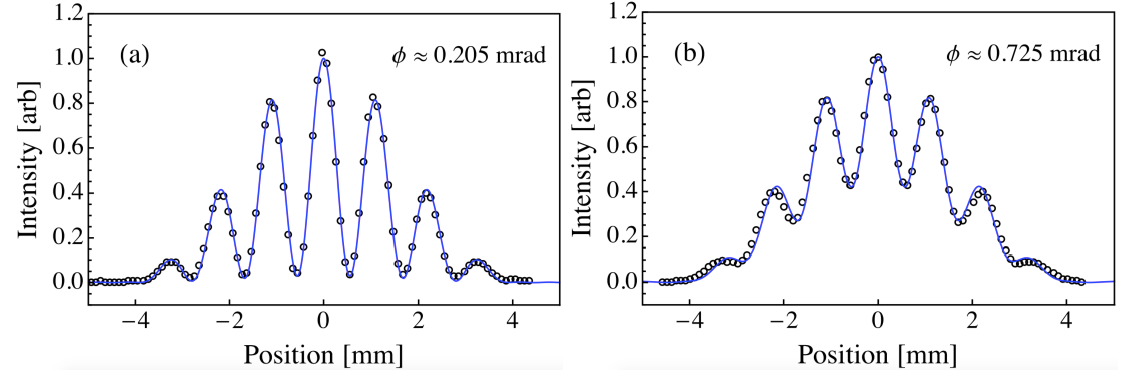
\includegraphics[]{dm8fig/dm8fig1.png}}
        
        \resizebox{\linewidth}{!}{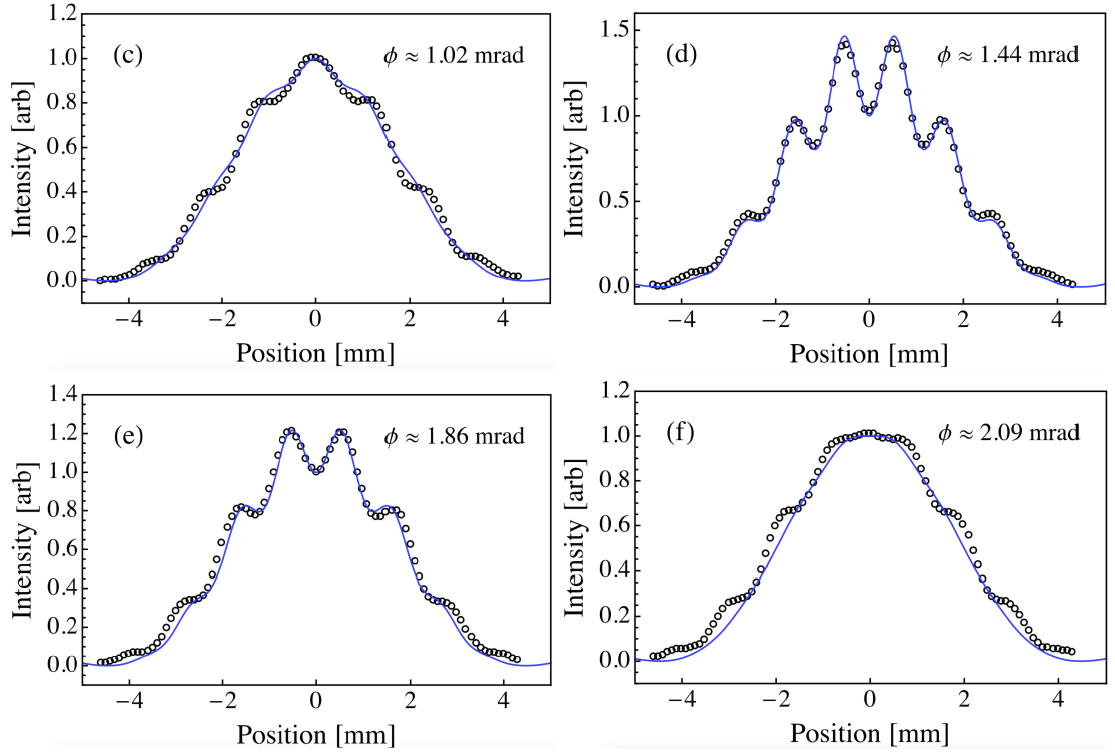
\includegraphics[]{dm8fig/dm8fig2.png}}
    \end{center}
    
    \begin{enumerate}[resume]
        \item À partir des documents, estimer la distance $a$ entre les deux fentes. Les résultats observés sont-il compatibles avec critère de brouillage ? Estimer la largeur $\epsilon$ des fentes utilisées.
    \end{enumerate}
    
    
\end{document}